\documentclass[a4paper]{article}
\usepackage[pdftex]{graphicx}
\usepackage[utf8]{inputenc}
\usepackage{enumerate}
\usepackage{siunitx}
\sisetup{locale=DE} 
\usepackage{icomma}
\usepackage{amssymb}
\usepackage{tikz}
\usepackage{href-ul}
\hypersetup{
	colorlinks=true,
	linkcolor=blue,
	urlcolor=blue}
\usepackage{geometry}
\geometry{a4paper, top=15mm, left=15mm, right=15mm, bottom=15mm,
	headsep=10mm, footskip=12mm}

\begin{document}
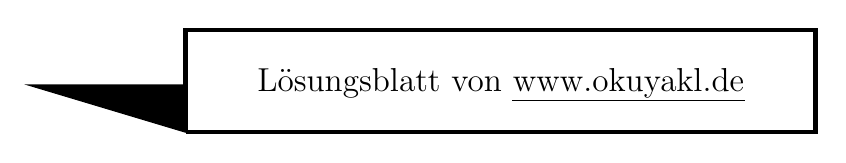
\begin{tikzpicture}(10,3)
	\draw[ultra thick](2,0) --(10,0) -- (10,1.3) --(2,1.3) -- (2,0);
	\draw[fill=black](2,0)-- (0,.6) -- (2,.6) -- (2,0);
	\node at (6,.6) {\large Lösungsblatt von \href{https://www.okuyakl.de}{www.okuyakl.de}};
\end{tikzpicture}
\vspace{0.5 cm}

\noindent{\bf Aufgabe 1.}\\
Massen sind träge, das bedeutet, dass sie ihren Bewegungszustand nur ändern, wenn eine Kraft auf sie wirkt. Zum Beispiel wenn eine Masse in Ruhe ist, dann setzt sie sich nicht ,,von alleine" in Bewegung, hierzu wäre eine Krafteinwirkung nötig.    
\vspace{0.5 cm}

\noindent {\bf Aufgabe 1. b)}\\
Der Grund, warum die Pedalkraft nicht zur immer weiteren Beschleunigung des Fahrradfahrers führt, liegt daran, dass Reibungskräfte, hauptsächlich der Luftwiderstand, entgegenwirken.
\vspace{0.5 cm}

\noindent {\bf Aufgabe 1. c)}\\
Zuerst bewegt sich der Schuh mit dem an ihm haftenden Schnee abwärts. Beim Auftreffen auf den Boden wird der Schuh stark abgebremst. Aufgrund der Trägheit ,,will" sich der Schnee jedoch weiter abwärts bewegen und löst sich von dem Schuh.
\vspace{0.5 cm}

\noindent {\bf Aufgabe 2. a)}\\
Wir berechnen schrittweise die auftretenden Kräfte von links nach rechts. Die Kraft am rechten Hebelarm ist: 
$$F_2=F_G \cdot {a_1 \over a_2}=\SI{1500}{\newton} \cdot {\SI{1,50}{\meter} \over \SI{2,50}{\meter} }=\SI{900}{\newton}$$
Die Seilkraft $F_s$ beträgt die Hälfte davon, also $$F_s=\SI{450}{\newton}$$
\vspace{0.5 cm}

\noindent {\bf Aufgabe 2. b)}\\
Die Kraft an der Kurbel ist gemäß Hebelgesetz:
$$F_k = F_s \cdot {a_s \over a_k}=\SI{450}{\newton} \cdot {\SI{0,10}{\meter} \over \SI{0,40}{\meter} }=\SI{112,5}{\newton}$$
\vspace{0.5 cm}

\noindent {\bf Aufgabe 2. c)}\\
Auf die Seilverankerung A wirkt die Hälfte der Kraft $F_2$. Also setzen wir  
$$F_2=2\cdot \SI{600}{\newton}= \SI{1200}{\newton}$$
Nun berechnen wir den Hebelarm $a_1$:
$$a_1 = a_2 \cdot {F_2 \over F_G}=\SI{2,50}{\meter}\cdot {\SI{1200}{\newton}\over \SI{1500}{\newton}}=\SI{2,0}{\meter}$$
\vspace{0.5 cm}

\noindent{\bf Aufgabe 3. a)}\\
Die Kraft auf den Nagel ist:
$$ F_2 = {{a_1 \over a_2} \cdot F_1} = {\SI{0,15}{\meter} \over \SI{0,035}{\meter}} \cdot \SI{180}{\newton} = \SI{771}{\newton}$$
\vspace{0.5 cm}

\noindent{\bf Aufgabe 3. b)}\\
Drehmoment links: 
$$ M_1 = F_1 \cdot a_1 = \SI{6,0}{\newton} \cdot \SI{0,030}{\meter}=\SI{0,18}{\newton\meter} $$
Drehmoment rechts: 
$$ M_2 = F_2 \cdot a_2 = \SI{3,0}{\newton} \cdot \SI{0,080}{\meter} = \SI{0,24}{\newton\meter} $$
Das verbleibende Moment ist die Differenz davon, also
$$ M_v = (0,18-0,24)\SI{}{\newton\meter} = \SI{0,06}{\newton\meter}$$
\begin{minipage}{0.5\textwidth}	
	Dies kann durch eine zusätzliche Kraft aufgehoben werden, die folgender Gleichung genügt: 
	$$ F_3 \cdot a_3 = \SI{0,06}{\newton\meter}$$
	Also z.B. 
	$$F_3 =\SI{3}{\newton}; \quad a_3 =\SI{0,02}{\meter}$$ 
	Diese Kraft muss z.B. rechts vom Lager angreifen und nach oben gerichtet sein, da das Moment rechts größer ist und dadurch geschwächt werden muss.
\end{minipage}
\hfill
\begin{minipage}{0.5\textwidth}
	\includegraphics[width= 6 cm]{hebgg406}
\end{minipage}


\vspace{0.5 cm}

\noindent{\bf Aufgabe 4. a)}\\
Durch die lose Rolle wird die Kraft halbiert, durch die feste Rolle nur umgelenkt. Also ist die Kraft im Punkt C: 
$$ F = {\SI{100}{\newton} \over 2} = \SI{50}{\newton}$$
\vspace{0.5 cm}

\noindent{\bf Aufgabe 4. b)}\\ 
Im Aufhängepunkt A wirkt die halbe Gewichtskraft, also $F_A=\SI{50}{\newton}$, im Punkt B wirkt diese halbe Kraft zweimal, also ist $F_B=\SI{100}{\newton}$.

\begin{center}
	\includegraphics[width=7 cm]{../../viecher/endcomic.pdf}
	
	Hier geht es zurück zum \href{https://www.okuyakl.de/phys/p8mecL406/aa406.pdf}{Aufgabenblatt}
\end{center}

\end{document}

